\documentclass[a4paper]{article}
\usepackage{fontspec}\defaultfontfeatures{Ligatures=TeX}
\usepackage{setspace}\setstretch{1.1} % \begin{spacing}{1.3}
\usepackage[a4paper,vmargin={3cm,3cm},hmargin={3cm,3cm}]{geometry}
%<--------------------------------------------------------------------------->%
\usepackage{settings}
%<--------------------------------------------------------------------------->%
%%% Title %%%
\title{How to compare the size of covariance matrices?}
\author{\href{https://jessekelighine.com}{\texttt{jessekelighine.com}}}
\date{\today}
%<--------------------------------------------------------------------------->%

\begin{document}

\maketitle

\begin{multicols}{2}

\noindent
Consider two covariance matrices $\AA_{n\times n}$ and $\BB_{n\times n}$.
We say that $\AA$ is \emph{bigger} than $\BB$,
often denoted by $\AA\geq \BB$ or $\AA\succsim \BB$, if $\AA-\BB$ is semi-positive definite.
Why do we use the ``definiteness'' of a matrix to compare the size of two covariance matrices?

First, notice that a covariance matrix is not only symmetrical, but also
semi-positive definite.  Consider a random vector $\xx=(x_1,...,x_n)\T$.
The covariance matrix is defined by
\begin{align*}
	\KK &\coloneqq \E{(\xx-\E{\xx})(\xx-\E{\xx})\T}.
\end{align*}
Given any constant vector $\vv$ of length $n$, we have
\begin{align*}
	\vv\T \KK \vv &= \E{\vv\T(\xx-\E{\xx})(\vv\T(\xx-\E{\xx}))\T} \geq 0
\end{align*}
by the definition of $\KK$.
Therefore, the covariance matrix $\KK$ is semi-positive definite.
In fact, $\vv\T\KK\vv$ is zero iff $\xx$ has no variance at all.

There is another intuitive way of interpreting the definiteness described above.
Consider the same vector $\vv$ and the random vector $\xx$.
The dot product $\vv\T \xx$ is the projection of the random vector from $n$-dimensional
space on a one-dimensional space along the direction of $\vv$, i.e.,
this collapse the $n$-dimensional random variable to a one-dimensional random variable through some linear combination.
If we calculate the variance of the one-dimensional random variable $\vv\T \xx$, we obtain
\begin{align*}
	\var{\vv\T \xx}
	&= \E{\vv\T \xx(\vv\T \xx)\T } - \E{\vv\T \xx}\E{\vv\T \xx}\T  \\
	&= \vv\T \big(\E{\xx\xx\T } - \E{\xx}\E{\xx}\T \big)\vv \\
	&= \vv\T \KK\vv.
\end{align*}
Notice that the variance assumes the exact form as before.
And since variance is non-negative, it is clear that the covariance matrix must be semi-positive definite.
That is, for any direction $\vv$,
the variance of ``$\xx$ projected on that direction'' is (clearly) non-negative.

Motivated by the intuitive interpretation, lets now compare two covariance matrices.
Let $\xx=(x_1,...,x_n)\T$ and $\yy=(y_1,...,y_n)\T$ be random vectors with mean $(0,...,0)\T$ for simplicity.
Let $\AA=\E{\xx\xx\T}$ and $\BB=\E{\yy\yy\T}$ be the covariance matrices.
Our goal is to compare $\AA$ and $\BB$ in some meaningful way.
We can project $\xx$ and $\yy$ on a vector $\vv$,
and then compare the variance (non-negative real number) of the two projections.
To make the comparison meaningful,
it is reasonable to compare \emph{all} possible projections,
i.e., consider all possible choices of $\vv$.

Formally, consider any vector $\vv$.
The projection of $\xx$ on $\vv$ is $\vv\T \xx$.
The variance of $\vv\T \xx$ is 
\begin{align*}
	\E{(\vv\T \xx)^2}
	&= \E{\vv\T \xx\xx\T\vv} \\
	&= \vv\T\E{\xx\xx\T}\vv
	= \vv\T \AA\vv
\end{align*}
where $\AA$ is the covariance matrix.
Similarly, consider the same for $\yy$.
If we find that $\forall\vv$,
\begin{align*}
	\vv\T \AA\vv - \vv\T \BB\vv
	= \vv\T (\AA - \BB)\vv
	\geq 0,
\end{align*}
then, by definition, $\AA-\BB$ is semi-positive definite.
Now we know why we say $\AA$ is \emph{larger} than $\BB$ when $\AA-\BB$ is positive definite:

\begin{tcolorbox}[enhanced,sharp corners,frame hidden,boxrule=0sp,borderline west={3pt}{0pt}{black!70}]
	If $\AA-\BB$ is positive definite,
	then \emph{for all possible directions $\vv$},
	the variance of $\xx$ is larger than $\yy$'s.
	\footnote{
	This order of semi-positive definite matrices is called the
	\href{https://en.wikipedia.org/wiki/Loewner_order}{L\"{o}wner ordering}.
	}
\end{tcolorbox}

This interpretation of the partial ordering can be understood easily through visualisation.
The following are representations of the distributions $\xx$ and $\yy$ where the
two random vectors are two-dimensional:
\begin{center}
	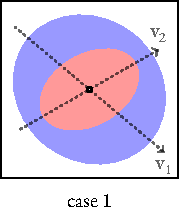
\includegraphics[width=0.2\textwidth]{figures/visual-1.pdf}
	\hspace{0.5em}
	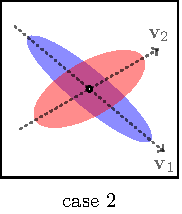
\includegraphics[width=0.2\textwidth]{figures/visual-2.pdf}
\end{center}
Let $\xx$ with covariance matrix $\AA$ be the blue distribution and $\yy$ with
covariance matrix $\BB$ be the red distribution.
It is clear that in case 1, $\AA$ is \emph{bigger} than $\BB$ since the variance of $\xx$ is
bigger that $\yy$'s in \emph{every} direction. (every possible direction of projection)
However, the same statement is not true in case 2.
In some directions (e.g.\! $\vv_1$), the variance of $\xx$ is larger;
in other directions (e.g.\! $\vv_2$), the variance of $\yy$ is larger.
Thus, $\AA$ and $\BB$ are not comparable by the partial order in case 2.
\asDemonstrated

\end{multicols}

\end{document}
